\chapter{La atm\'osfera}
 
 La capa gaseosa que rodea la Tierra se le conoce como atm\'osfera, los planetas peque\~nos poseen menos atmósfera por que tiene menos masa. En la Tierra la  mayor parte de la masa se acumula en los primeros 11 \kilo\metre\,  de altura (aproximadamente el 95\% del aire se ubica en la primera capa). Los gases son atra\'{\i}dos por la gravedad y se mantienen debido a \'esta, si la gravedad no es suficiente la atm\'osfera es barrida por el viento solar, como ocurre en otros planetas.


 \section{Estructura de la Atm\'osfera}
  Las capas de la atm\'osfera son las siguientes y se pueden ver en la figura~\ref{capasATM} :


\textbf{Exosfera}  se encuentra ubicada a 500\kilo\metre\, posee \'atomos y mol\'eculas no unidas por la gravedad.

\textbf{ Term\'osfera }entre 400 a 500\kilo\metre, $10^6$ -- $10^{14}$ menos denso que en la superficie. 1,000 -- 2,000\kelvin. Se encuentran \'atomos de \ce{O2}, \ce{N2}. La qu\'{\i}mica se rige por la luz ultravioleta $\lambda\leqq 150$nm. $\alpha,\beta$ 121.6$\nano\metre$ 102.6\nano\metre. En esta capa se encuentran  rayos X.
 
 \textbf{Mesosfera} de 50-100$\kilo\metre$  ($\pm10$). La concentraci\'on de mol\'eculas va de 10$^{13}$--10$^{16}$ molec/cc. La temperatura va de los 130 -- 250 \kelvin. L qu\'{\i}mica es dirigida por luz ultravioleta $\lambda=250\nano\metre$. Se encuentran mol\'eculas simples \ce{O2}, \ce{N2}, \ce{CO2}, \ce{H2O}, \ce{O3}, radicales como \ce{OH}, \ce{HO2} iones \ce{O2-},\ce{NO2-}
 
 \index{atmosfera@atmósfera!estructura}
\begin{wrapfigure}[25]{r}{35mm}
\centering
%\begin{figure}[htbp]
%\begin{center}
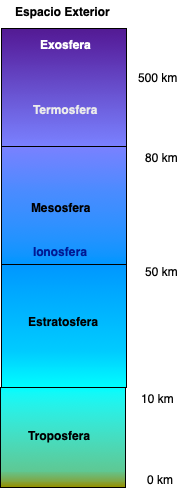
\includegraphics[width=0.30\textwidth]{atmosfera_capas.png}
 %\vspace{-110pt}
\caption{Capas de la atm\'osfera}
\label{capasATM}
%\end{center}
%\end{figure}
\end{wrapfigure}
 \textbf{Ionosfera} Sobre 60 \kilo\metre. Se encuentran electrones libres cuya concentraci\'on puede alcanzar $10^6$molec/cc. En esta capa se da la propagaci\'on de las ondas de radio.
 
 \textbf{Estratosfera} Como su nombre lo indica esta en capas de $10-17 \kilo\metre$ hasta $50\kilo\metre$. El mezclado vertical toma a\~nos. La qu\'{\i}mica es dirigida por luz ultravioleta, visible con longitudes de onda mayores a los 175\nano\metre. Existen mol\'eculas mas complejas \ce{HNO3}, \ce{HO2}, \ce{NO2}, \ce{CH3O2}, \ce{ClONO2}, etc. Posee algunas nubes.
 
 \textbf{Troposfera} De la superficie a $10-17\kilo\metre$. El mezclado vertical es r\'apido de minutos a d\'{\i}as. La temperatura oscila de $200-300$  \kelvin. Hay mol\'eculas complejas hasta de cerca de \ce{C12H26} en fase gaseosa.

  \section{Composición de la Atmósfera}
 \index{atmosfera@atmósfera!composicion@composición}

La composición de la atmósfera ha variado desde el origen de la Tierra, al principio existían óxidos de azufre los cuales fueron reemplazados por oxígeno generado por las plantas. Posteriormente procesos biológicos como la descomposición de la materia orgánica, erupciones volcánicas, incendios de bosques y procesos biológicos de organismos en el mar y tierra han contribuido en cambios en la composición de la atmósfera.  En zonas no contaminadas se considera que los principales constituyentes son el nitrógeno (\ce{N2}), el  oxígeno (\ce{O2}), el argón (Ar ), y el bióxido de carbono (\ce{CO2}) las proporciones se muestran en el \textbf{Cuadro~\ref{Atmcomp}}.

\begin{table}[htp]{\small 
\caption{Composición de la atmósfera (\mole/\mole)}
\begin{center}
\begin{tabular}{|l|l|l|l|}\hline
Compuesto & Fracción & Compuesto & Fracción\\ \hline\hline
Nitrógeno (\ce{N2})   & 0.78   &  Ozono (\ce{O3})  & 0.01-10$\times$10$^{-6}$ \\
Oxígeno (\ce{O2})    & 0.21   &  Helio  (\ce{He})    & 5.6$\times$10$^{-6}$ \\
Argón (\ce{Ar})    & 0.0093   &  Metano  (\ce{CH4})    & 1.7$\times$10$^{-6}$ \\
Dióxido de Carbono (\ce{CO2})    &   390$\times$10$^{-6}$ &  Kripton  (\ce{Kr})    & 1.1$\times$10$^{-6}$ \\
Neón (\ce{Ne})    &   18$\times$10$^{-6}$ &  Hidrógeno  (\ce{H})    & 500$\times$10$^{-9}$ \\\hline
\end{tabular}
\end{center}
\label{Atmcomp}}
\end{table}%



\section{El ozono } \index{ozono}
 \label{esozono}
El ozono (\ce{O3}) es una forma alotr\'opica del ox\'{\i}geno (\ce{O2}) que esta constituido por tres \'atomos de ox\'{\i}geno. Se encuentra en la estratosfera, a una altura de entre 20 y 30 \kilo\metre , donde forma la capa de ozono (\textbf{Figura~\ref{atmoO3}}).

Esta capa absorbe a los rayos ultravioleta del Sol. Si esa acci\'on, los rayos solares podr\'{\i}an causar c\'ancer de piel, mutaciones y deficiencias inmunitarias. 

El ozono estratosf\'erico se ve afectado por los cloro fluorocarbonos (CFC). Estos compuestos son inertes en la troposfera y debido a ello se desplazan hacia la estrat\'osfera. En el polo Sur mediante procesos catal\'{\i}ticos 

\begin{figure}[htbp]
\begin{center}
\begin{picture}(75,72)
% Cuadro
\put(10,7){\line(1,0){55}}
\put(10,67){\line(1,0){55}}
\multiput(20, 7)(10,0){5}{\line(0,1){2}}
\put(10,7){\line(0,1){60}}
\put(65,7){\line(0,1){60}}
\multiput(10,15)(0,10){6}{\line(1,0){2}}
% numeros horizontal
\put(19,3){1}
\put(29,3){2}
\put(39,3){3}
\put(49,3){4}
\put(59,3){5}
\put(30,0){\footnotesize$\times10^{12}$  molec/cm$^3$}
% numeros vertical
\put(6,6){0}
\put(4,16){10}
\put(4,26){20}
\put(4,36){30}
\put(4,46){40}
\put(4,56){50}
\put(4,66){60}
\put(4,70){\kilo\metre}

%

\put(28,45){\footnotesize Estratosfera}
\put(28,14){\footnotesize Troposfera}
\put(0,26){\shortstack{A\\l\\t\\i\\t\\u\\d}}
\thicklines
\qbezier(10,55)(12,47)(30,38)
\qbezier(30,38)(36,34)(55,30)
\qbezier(55,30)(65,27) (55,24)
\qbezier(32,20)(35,21) (55,24)
\qbezier(18,7)(18,17)(32,20)

\dashline[+30]{3}(10,19)(65,19)
\dashline[+30]{3}(10,55)(65,55)
\end{picture}

\caption[Variación de ozono en la atmósfera]{Variación de la concentración de ozono en las diferentes capas de la atmósfera.}
\label{atmoO3}
\end{center}
\end{figure}


 \section{Cambio Climático}
 \index{cambio climatico}
 
Una forma de distinguir entre clima y tiempo es tomar en cuenta que el clima\index{clima} es lo que deberíamos de tener y el tiempo es lo que tenemos. Así el clima fluctúa naturalmente entre períodos cálidos y fríos; sin embargo, en el siglo XX se ha visto el mayor calentamiento en los últimos mil años.
\subsection{Efecto invernadero}
\index{efecto invernadero}
La mayoría de la energía del Sol, conocida como radiación solar, se absorbe en la tierra, pero alguna se refleja hacia el espacio. Las nubes y los gases en la atmósfera absorben parte del calor de la Tierra, evitando que escape al espacio. Esto mantiene a nuestro planeta los suficientemente caliente para la existencia de la vida y es conocido como ``efecto invernadero''.

\subsection{Calentamiento Global}
\index{calentamiento global}
El efecto invernadero se puede incrementar si se incrementan ciertos gases, a esto se le conoce como ``calentamiento global''.
Algunos de los compuestos que contribuyen al calentamiento global  \ce{CO2}, \ce{CH4}, partículas (hollín), \ce{N2O}, compuestos fluorados y \ce{O3}.
\begin{itemize}
\item  Entre hace 1,500 a 1,100 millones de años se encuentra un brusco cambio climático global, debido a un cambio en la composición de la atmósfera que la hizo ser de reductora a oxidante.
\item  En periodos posteriores se encuentran también cambios climáticos en el precámbrico. A lo largo del Proterozoico se describen diversos procesos glaciares de los cuales al menos dos tienen evidencias concretas para soportarse. 
\item  Se piensa que estas glaciaciones ocurrieron principalmente por el importante aumento de oxígeno y vapor de agua en la atmósfera provocado por la actividad vegetal de la época. 
\item  Los cambios climáticos que se efectúan en la Tierra de forma natural han llegado a ser desbastadores, hasta poner en crisis a la vida misma al tener extinciones casi masivas de fauna.
\item  Un ejemplo de lo anterior ocurrió a finales del Paleozoico en donde se cree que estos cambios bruscos de clima se produjeron a partir de cambios paleogeográficos, es decir, cuando las masa continentales se reunieron en un supercontinente.
\item  Durante la era Mesozoica existieron grandes cambios climáticos de igual manera. Esta era comienza con un clima árido seguido por otro muy cálido en el cual no se pueden definir estaciones. 
\item  Estos cambios climáticos así como movimientos tectónicos, provocaron que las tierras emergidas quedaran inundadas como islotes a consecuencia de la expansión de los mares en donde también comenzó la fragmentación del supercontinente ``Pangea''. La era Mesozoica finalizó con un brusco enfriamiento del clima, lo que produjo nuevas extinciones masivas.
\end{itemize}

\subsection{Señales del cambio climático}

El incremento de la temperatura global se manifiesta a través de diversas señales observables en el sistema climático. Algunas de las más significativas incluyen:

\begin{description}
    \item[Incremento en la concentración de \ce{CO2}] En las últimas décadas, se ha registrado un aumento sostenido en la concentración de \ce{CO2}, lo que está estrechamente relacionado con el incremento de la temperatura ambiental debido al efecto invernadero.
    
    \item[Calentamiento de los océanos] El aumento de la temperatura en los océanos implica una mayor acumulación de energía térmica en el agua de mar, lo que afecta los patrones climáticos y la biodiversidad marina.
    
    \item[Reducción de los glaciares] La extensión de los glaciares ha disminuido considerablemente en las últimas décadas, evidenciando el calentamiento global y afectando el equilibrio hídrico de diversas regiones del planeta.
    
    \item[Blanqueamiento de los corales] El incremento de la temperatura del agua de mar provoca la expulsión de las algas simbióticas de los corales, responsables de su coloración. Si este fenómeno persiste, los corales no logran recuperarse, lo que compromete su supervivencia y afecta los ecosistemas marinos.
    
    \item[Aumento del nivel del mar] El derretimiento de los hielos continentales y la expansión térmica del agua de los océanos provocan un incremento en el nivel del mar, lo que genera la pérdida de áreas costeras, un incremento en la erosión de playas y mayores riesgos para las comunidades costeras.
\end{description}

\subsection{Ciclos de la Tierra}

La órbita de la Tierra alrededor del Sol y su orientación cambian de manera regular, lo que provoca variaciones en la cantidad de radiación solar que alcanza la superficie terrestre. Estos cambios cíclicos están asociados con períodos de calentamiento y glaciaciones. 

\begin{itemize}
    \item Bamboleo del eje giratorio: 13 - 23 mil años.
    \item Inclinación del eje rotatorio: 41 mil años.
    \item Variaciones en la órbita de la Tierra: 125 y 400 mil años.
\end{itemize}

Durante los períodos de glaciación, los niveles de \ce{CO2} disminuyen significativamente. Sin embargo, las emisiones continuas de gases de efecto invernadero podrían aumentar la temperatura global entre 1 y 5 \celsius\, para el año 2100. Este incremento térmico podría desencadenar eventos climáticos extremos, como sequías e inundaciones, así como el aumento del nivel del mar, amenazando los recursos costeros y los humedales.

Además, el cambio climático incrementaría el riesgo de propagación de enfermedades debido a la aparición de nuevos hábitats propicios para pestes y patógenos. Asimismo, la degradación de los ecosistemas conduciría a una reducción de la biodiversidad, afectando el equilibrio de los sistemas naturales.

\subsection{Forzamiento radiativo}

El forzamiento radiativo se define como el cambio en la irradiación neta vertical (expresada en \wattpersquaremetrenp) en la tropopausa debido a una variación interna del sistema climático o a un forzamiento externo, como el aumento en la concentración de dióxido de carbono o las variaciones en la potencia del Sol \textbf{(Figura~\ref{CGWP})}. 

Generalmente, el forzamiento radiativo se calcula tras permitir que las temperaturas estratosféricas alcancen un nuevo equilibrio radiativo, mientras que las propiedades de la troposfera se mantienen constantes en sus valores originales, sin perturbaciones. 


\begin{figure}[!htbp]
\begin{center}
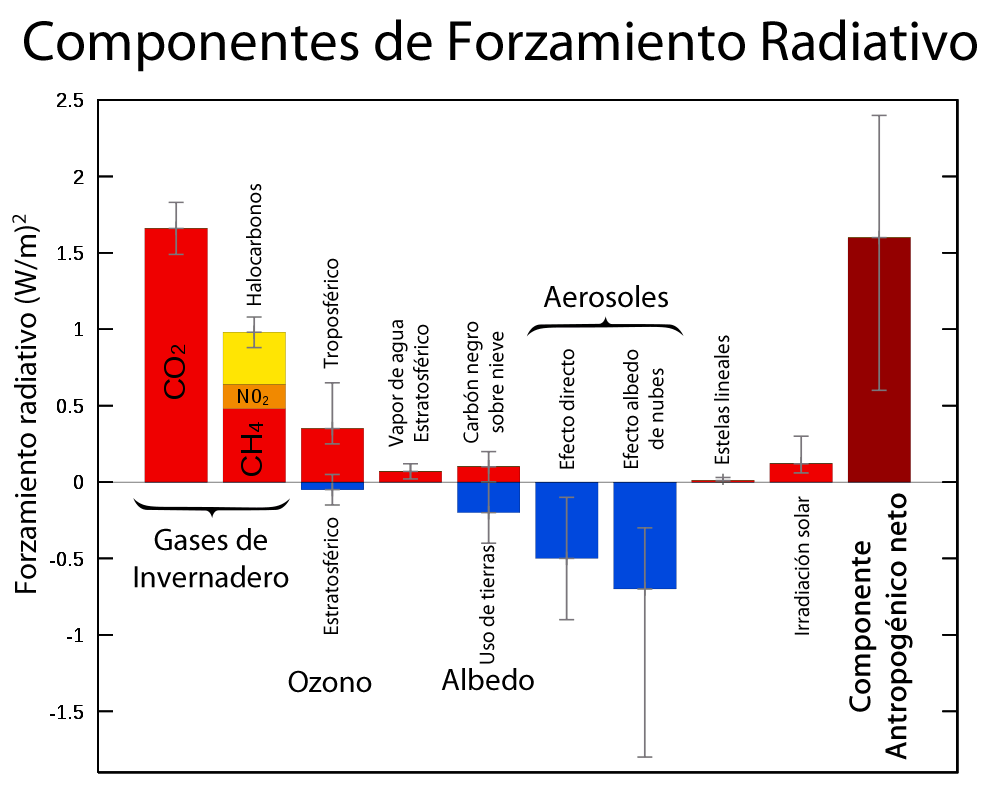
\includegraphics[width=0.8\textwidth]{forzantes-radiativos.png}
\caption{Forzamiento radiativo de componentes atmosféricos.}
\label{CGWP}
\end{center}
\end{figure}

Dependiendo del compuesto, su capacidad de absorción de radiación determina su potencial de calentamiento global, el cual se muestra en el \textbf{Cuadro~\ref{WGP}} (IPCC, \textup{4\textsuperscript{to}.} informe, 2007).


\begin{table}[htp]
\caption{Potencial de Calentamiento de varios compuestos}
\begin{center}
{\small \begin{tabular}{|l|l|r|r|r|}\hline
Nombre & Fórmula & Vida    & \multicolumn{2}{c}{Potencial Calentamiento Global} \\
común  & química  & (años) &  100-años & 20 años \\\hline\hline
Dióxido de carbono & \ce{CO2} &       & 1   & 1 \\
Metano                    &  \ce{CH4} & 12 & 25 &72 \\
Oxido nitroso          &  \ce{N2O}  & 114& 289 &298\\  \hline
\multicolumn{5}{l}{Sustancias controladas por el Protocolo de Montreal}\\ \hline
CFC-11                  & \ce{CCl3F}    & 45   &  6,730 & 4,750 \\
CFC-12                 & \ce{CCl2F2}  & 100 &11,000 & 10,900 \\
CFC-115                & \ce{CClF2CF3}  &1,700 &5,310 & 7,370 \\
Halon-11301          & \ce{CBrF3}    & 65  & 8,480 & 7,140 \\
Tetracloruro de Carbono & \ce{CCl4} & 26 & 2,700 & 1,400 \\
Bromuro de metilo & \ce{CH3Br} & 0.7  &17 & 5 \\
HCFC-22               & \ce{CHClF2} & 12 & 5,160 & 1,810 \\
HCFC-123             & \ce{CHCl2CF3} & 1.3 & 273 & 77       \\ \hline
\multicolumn{5}{l}{Hidrofluorcarbonos}\\\hline
HFC-23                  &\ce{CHF3}  & 270 & 12,000 & 14,800 \\
HFC-32                  &\ce{CH2F3}  & 4.9 & 2,330 & 675 \\
HFC-125                & \ce{CHF2CF3} & 29 & 6,350 & 3,500 \\
HFC-134a              & \ce{CHFCF3} & 14 & 3,830 & 1,430 \\
HFC-236fa            & \ce{CF3CH2CF3} & 240 & 8,100 &9,810 \\ \hline
\multicolumn{5}{l}{Compuestos Perfluorinados}\\\hline
Hexafloruro de azufre & \ce{SF6}   & 3,200  & 16,300 &22,800 \\
Trifloruro de nitrógeno & \ce{NF3}  & 740     & 12,300 & 17,200 \\
PFC-14                        &\ce{CF4}   &50,000 & 5,210   &   7,390\\
PFC-116                        &\ce{C2F6}   &10,000 & 8,630 & 12,200\\ \hline
\end{tabular}}
\end{center}
\label{WGP}
\end{table}%


